% Mirror: https://github.com/SIGma-UIUC/presentation-format
% --------------------------------------------------------------------
% This is a simple Beamer document that uses beamerthemesigma.sty
% Reading the comments should help you create a presentation even if
% you've never used Beamer before.
% --------------------------------------------------------------------

% Set our document class to Beamer
\documentclass[aspectratio=169]{beamer}
% \documentclass[aspectratio=169, handout]{beamer}
% Add handout option to ignore pauses

% From Jeff E
\usepackage{algo}
% Some more macros
\usepackage{sigmastyle}

\declaretheorem[style=solution, numbered=no, name=``Proof'' by Picture]{pf_pic}


% Set a title
\title{Cuckoo Hashing}

% Set a subtitle if you desire
% \subtitle{[TAOCP 5 8.9.10.11]}

% Whoever worked on the presentation:
\author{Alex Broihier}

% Date looks ugly, so leave blank
\date{}

% An institute name, if you're so inclined
% \institute{University of Illinois Urbana-Champaign}

% Use the SIGma theme for this Beamer presentation
\usetheme{sigma}
% --------------------------------------------------------------------

% Begin document
\begin{document}

% Beamer calls each slide a "frame", defined within the environment:
% \begin{frame}
%   <frame content here>
% \end{frame}

% This frame is just the title.
\begin{frame}
\titlepage
\end{frame}

% A frame with the table of contents.
% This frame's title is "Outline".
\begin{frame}{Outline}
  \tableofcontents
\end{frame}

\section{Hashing Functions and Families}
\frame{\sectionpage}

\begin{frame}{Hash Functions}
    \begin{itemize}
        \item $h$ is a hash function if it has the form $h: U \to \{0, 1, \ldots, n - 1\}$ for some set $U$ and some constant $n$
        \item Example: if $U$ is the integers, $h(x) = x \text{ mod } n$ is a hash function \pause
        \item Often used to assign an element an index in an array of size $n$
        \item This alone is not useful; hash functions are typically used to take an arbitrarily input and give back a seemingly random output
    \end{itemize}
\end{frame}

\begin{frame}{Hash Families}
    \begin{itemize}
        \item A hash family is a set of hash functions, $\{h_1, h_2, \ldots\}$
        \item They provide a source of randomness: you can randomly sample a hash function to use from a hash family \pause
        \item This will allows us to analyze hash families probabilistically
    \end{itemize}
\end{frame}

\begin{frame}{Universal Hash Families}
    \begin{itemize}
        \item A universal hash family is a hash family with the property
        \begin{align*}
            Pr_{h \in H}[h(x) = h(y)] \le \frac 1 n \quad\quad x \ne y
        \end{align*}
    \end{itemize}
    \nocite{overview}
    \nocite{site:jeff}
\end{frame}

\begin{frame}{$(c, k)$ Universal Hash Families}
    \begin{itemize}
        \item We can generalize universal hash families (and get stronger guarantees while we are at it)
        \item A hash family is $(c, k)$ universal if for all $x_1, x_2, \ldots, x_k \in U$ and for all $y_1, y_2, \ldots, y_k \in \{0, 1, \ldots, n - 1\}$
        \begin{align*}
            Pr_{h \in H}[h(x_1) = y_1, h(x_2) = y_2, \ldots, h(x_k) = y_k] \le \frac c {n^k}
        \end{align*} \pause
        \item The previously discussed ``standard'' universal hash family is $(1, 2)$ universal
    \end{itemize}
\end{frame}

\begin{frame}{Aside: Amortized vs Expected Cost}
    \begin{itemize}
        \item Randomness is present in our hashing algorithms, so we need the language to properly describe this. Amortized and expected runtime are different things. \pause
        \item Amortized runtime is guaranteed to ``average out.'' We analyze the runtime across numerous runs (even though a worst case individual run could be expensive)
        \begin{itemize}
            \item Example: push back for a dynamically sized array takes amortized $O(1)$ time
        \end{itemize} \pause
        \item Expected runtime is what will probably happen. The absolute worst case can be very bad (but will very rarely occur)
        \begin{itemize}
            \item Example: quicksort with randomized pivots takes expected $O(n \text{log} n)$ time
        \end{itemize}
    \end{itemize}
\end{frame}

\section{Hash Tables and Hashing Strategies}
\frame{\sectionpage}

\begin{frame}{Hash Tables}
    \begin{itemize}
        \item A hash table uses hashing to implement a ``dictionary'' data structure, which uses keys to access values \pause
        \item Fundamental Operations:
        \begin{itemize}
            \item Add key / value pair
            \item Lookup the value for a given key
            \item Remove key / value pair
        \end{itemize}
    \end{itemize}
\end{frame}

\begin{frame}{Hash Table Implementation}
    \begin{itemize}
        \item Use some hash function $h$ (may be randomly sampled from some hashing family)
        \item Store an array of size $r$ to hold $n$ elements; we keep $\frac n r \le C$, where $C$ is some constant and $\frac n r$ is the ``load factor''
        \item For each key / value pair, store it at index $h(\text{key}) \text{ mod } n$ \pause
        \item Hidden Operations:
        \begin{itemize}
            \item Rehash (resample hash function $h$)
            \item Resize (grow or shrink the internal array)
        \end{itemize} \pause
        \item What happens if two key / value pairs are assigned to the same index in our array?
    \end{itemize}
\end{frame}

\begin{frame}{Resolving Hash Table Collisions}
    \begin{itemize}
        \item We say a collision happened when more than one key / value pair is assigned to the same index
        \item Separate Chaining
        \begin{itemize}
            \item Store a linked list (or some other data structure) of key / value pairs at each index
            \begin{center}
                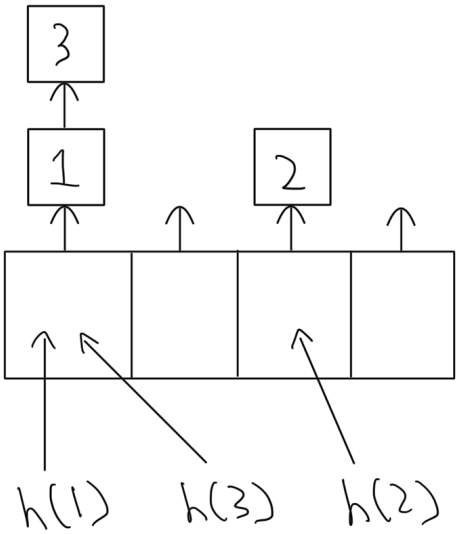
\includegraphics[width=0.3\textwidth]{images/sep_chain.png}
            \end{center}
        \end{itemize}
    \end{itemize}
\end{frame}

\begin{frame}{Resolving Hash Table Collisions (Continued)}
    \begin{itemize}
        \item We say a collision happened when more than one key / value pair is assigned to the same index
        \item (Linear) Probing
        \begin{itemize}
            \item Upon collision, keep searching until you find the first unoccupied entry in the array
            \begin{center}
                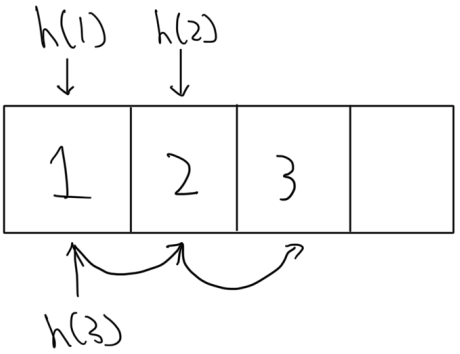
\includegraphics[width=0.4\textwidth]{images/lin_probe.png}
            \end{center}
        \end{itemize}
    \end{itemize}
\end{frame}

\begin{frame}{Separate Chaining Analysis}
    \begin{itemize}
        \item Insert is $O(1)$ time
        \item Lookup and Delete are expected $O(1)$ time \pause
        \begin{itemize}
            \item Lookup and Delete depend on how many elements are in the linked list at index $h(\text{key}) \text{ mod } n$
            \item If we treat $h$ as random (use a $(c, k)$ universal hash family), we would expect $\frac n r$ elements at each index \pause
            \item We bound our load factor above by a constant, so we can treat it as that upper bound
            \item Thus the linked list at index $h(\text{key}) \text{ mod } n$ has expected $O(1)$ elements, so lookup and delete are expected $O(1)$ time
        \end{itemize}
    \end{itemize}
\end{frame}

\begin{frame}{Linear Probing Analysis}
    \begin{itemize}
        \item Insert, Lookup, and Delete are expected $O(1)$ time \pause
        \begin{itemize}
            \item These all depend on the length of the chain starting at index $h(\text{key}) \text{ mod } n$
            \item Can show that the expected chain length is a linear function of $\frac n r$ (which we bound above)
        \end{itemize}
    \end{itemize}
\end{frame}

\section{Cuckoo Hashing}
\frame{\sectionpage}

\begin{frame}{Cuckoo Hashing}
    \begin{itemize}
        \item What if instead of storing one array, what if we store two arrays of length $r$? \pause
        \item Pick $r \ge (1 + \epsilon) n \implies \frac r n \ge 1 + \epsilon$
        \item Each array corresponds to one of two independent hash functions, $h_1$ and $h_2$, which are randomly sampled from hash family $H$
        \begin{center}
            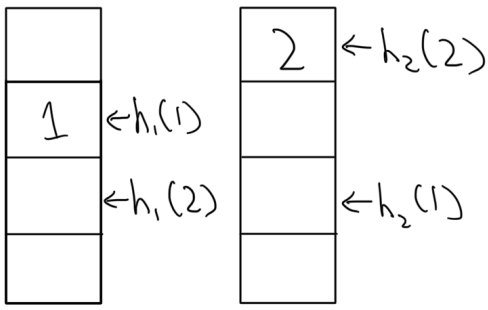
\includegraphics[width=0.4\textwidth]{images/cuckoo.png}
        \end{center}
    \end{itemize}
\end{frame}

\begin{frame}{Cuckoo Hashing: Lookup and Delete}
    \begin{itemize}
        \item To lookup a key, we use $h_1$ to index into the first array; if we don't find the key there, we use $h_2$ to index into the second array
        \item To delete a key, we follow a similar process \pause
        \item Importantly, we search at most two locations (one entry per array), so lookup and delete take worst case $O(1)$ time \pause
        \item But how does insert work?
    \end{itemize}
\end{frame}

\begin{frame}{Cuckoo Hashing: Insert}
    \begin{itemize}
        \item Hash the key using $h_1$ and check to see if the corresponding spot in the array is available
        \item If the location is occupied:
        \begin{itemize}
            \item Put our new key / value in the location, take the old key / value pair
            \item Hash the old key with $h_2$ to find its spot in the other array
            \item If the spot is in the other array is occupied, repeat this process (loop)
        \end{itemize}
        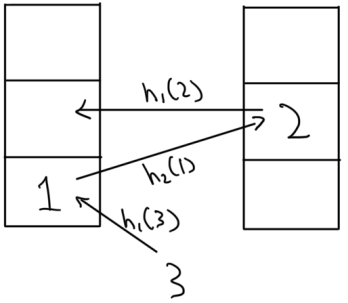
\includegraphics[width=0.25\textwidth]{images/insert1.png} \hspace{0.05\textwidth}
        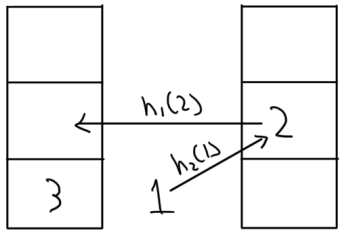
\includegraphics[width=0.25\textwidth]{images/insert2.png} \hspace{0.05\textwidth}
        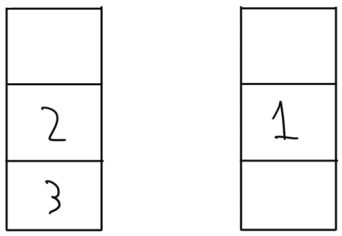
\includegraphics[width=0.25\textwidth]{images/insert3.png}
    \end{itemize}
\end{frame}

\begin{frame}{Cuckoo Hashing: Insert (Continued)}
    \begin{itemize}
        \item Problem: Insert could infinite loop
        \item Solution: If we loop more than $\emph{Max\_Loop} = 3 \text{log}_{1 + \epsilon}r$ times, rehash the entire table
    \end{itemize}
\end{frame}

\begin{frame}{Cuckoo Hashing: Insert (Continued)}
    \begin{itemize}
        \item Our present understanding: cuckoo hashing is good if we can afford costly inserts and want $O(1)$ time lookup and delete \pause
        \item Claim: cuckoo hashing insert is expected amortized $O(1)$ runtime
    \end{itemize}
\end{frame}

\begin{frame}{Insert Analysis}
    \begin{itemize}
        \item Let $h_1$ and $h_2$ be from a universal hash family $H$ that is at least as strong as ($1, \emph{Max\_Loop}$) universal
        \begin{itemize}
            \item Research has shown that with probability $1 - O(\frac 1 {n^2})$, we can treat $h_1$ and $h_2$ as independent random functions
        \end{itemize} \pause
        \item Let $x_1, x_2, \ldots, x_k$ be the sequence of keys we encounter during insert
        \begin{itemize}
            \item We call $x_1, x_2, \ldots, x_k$ nestless keys
        \end{itemize}
    \end{itemize}
\end{frame}

\begin{frame}{Insert Analysis (Continued)}
    \begin{itemize}
        \item Case 1: $x_1, x_2, \ldots, x_k$ are all distinct (and thus we have a finite sequence)
        \begin{center}
            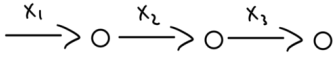
\includegraphics[width=0.75\textwidth]{images/case1.png}
        \end{center}
    \end{itemize}
\end{frame}

\begin{frame}{Insert Analysis (Continued)}
    \begin{itemize}
        \item Case 2: $x_1, x_2, \ldots, x_k$ has some repeated value $x_i = x_j, i \ne j$, but we have a finite sequence
        \begin{center}
            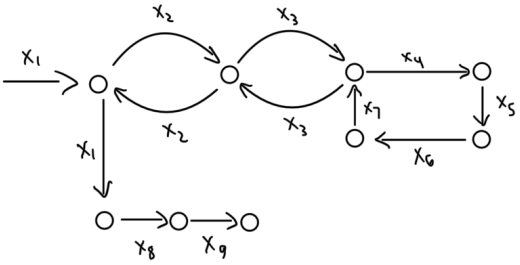
\includegraphics[width=0.75\textwidth]{images/case2.png}
        \end{center}
    \end{itemize}
\end{frame}

\begin{frame}{Insert Analysis (Continued)}
    \begin{itemize}
        \item Case 3: $x_1, x_2, \ldots, x_m, \ldots$ has some repeated values and forms an infinite sequence (so we need to rehash the table)
        \begin{center}
            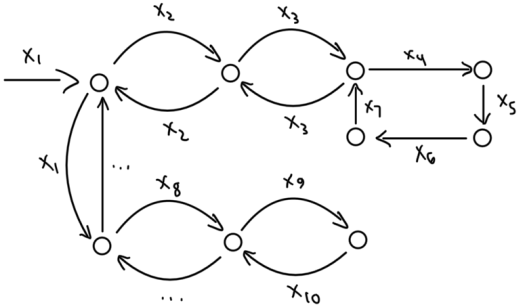
\includegraphics[width=0.75\textwidth]{images/case3.png}
        \end{center}
    \end{itemize}
\end{frame}

\begin{frame}{Insert Analysis (Continued)}
    \begin{itemize}
        \item With probability $1 - O(\frac 1 {n^2})$ we treat $h_1$ and $h_2$ as random functions and continue on with the analysis
        \item With probability $O(\frac 1 {n^2})$ the worst case might as well happen and we rehash
    \end{itemize}
\end{frame}

\begin{frame}{Insert Analysis: Lemma}
    \begin{lem}
        For a sequence of nestless keys that has not formed a closed loop, $x_1, \ldots, x_k$, there exists a consecutive subsequence $x_q, \ldots, x_{q + \ell - 1}$ of distinct keys where $x_1 = x_q$ and $\ell \ge \frac k 3$.
    \end{lem} \pause
    \begin{pf_pic}
        Worst case:
        \begin{center}
            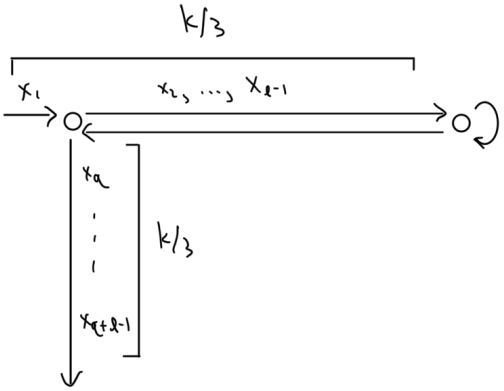
\includegraphics[width=0.45\textwidth]{images/proof.png}
        \end{center}
    \end{pf_pic}
\end{frame}

\begin{frame}{Insert Analysis: Cases 1 and 2 Bounds}
    \begin{itemize}
        \item By the previous lemma, there exists a sequence of at least $\frac k 3$ distinct nestless keys, $b_1, \ldots, b_v$
        \item Then $h_1(b_1) = h_1(b_2), h_2(b_2) = h_2(b_3), h_1(b_3) = h_1(b_4), \ldots$ (or same thing, but with $h_1$ and $h_2$ swapped) \pause
        \item Less than $n^{v - 1}$ ways to have $v$ distinct keys ($v - 1$ since we treat $x_1$ as fixed)
        \item Since we are treating $h_1$ and $h_2$ are random, each way to select the distinct keys has probability $r^{-(v - 1)}$
    \end{itemize}
\end{frame}

\begin{frame}{Insert Analysis: Cases 1 and 2 Bounds (Continued)}
    \begin{itemize}
        \item Recall that $\frac r n \ge 1 + \epsilon$
        \item Probability for this case is $2 n^{v - 1} r^{-v + 1} = 2 (\frac r n)^{-v + 1} \le 2 (1 + \epsilon)^{-\frac k 3 + 1}$
        \item Thus the probability that we get case 1 or 2 and see $k$ keys is at most $2 (1 + \epsilon)^{-\frac k 3 + 1}$
    \end{itemize}
\end{frame}

\begin{frame}{Insert Analysis: Case 3 Bounds}
    \begin{itemize}
        \item For a sequence of $k$ nestless keys with a closed loop, let $v$ be the number of distinct keys
        \item Once again, we have less than $n^{v - 1}$ way to chose the remaining distinct keys and $r^{v - 1}$ ways to put them in the table \pause
        \item There are at most $v^3$ ways to pick the start and end of the first loop and the start of the second loop \pause
        \item Each arrangement of nestless keys occurs with probability $r^{-2v}$ ($r^{-v}$ for each hash function)
    \end{itemize}
    \nocite{site:mit}
\end{frame}

\begin{frame}{Insert Analysis: Case 3 Bounds (Continued)}
    \begin{itemize}
        \item Altogether, the probability is bounded by
        \begin{align*}
            \Sigma_{v = 3}^{\ell}v^3 n^{v - 1}r^{v - 1}r^{-2v} &= \frac 1 {nr} \Sigma_{v = 3}^{\ell}v^3 n^{v}r^{v}r^{-2v} \\
            &\le \frac 1 {nr} \Sigma_{v = 3}^{\infty}v^3 (\frac r n)^{-v} \\
            &\le \frac 1 {nr} \Sigma_{v = 3}^{\infty}v^3 (1 + \epsilon)^{-v} \\
            &= \frac 1 {n O(n)} O(1) \\
            &= O(\frac 1 {n^2})
        \end{align*}
    \end{itemize}
\end{frame}

\begin{frame}{Insert Analysis (Continued)}
    \begin{itemize}
        \item We can now calculate an upper bound on the expected value for the number of nestless keys:
        \begin{itemize}
            \item $1$: there is always at least one nestless key \pause
            \item $\sum_{k = 2}^{2 * \emph{Max\_Loop}} 2(1 + \epsilon)^{-\frac k 3 + 1}$: case 1 or 2 with between $2$ and $2 * \emph{Max\_Loop}$ nestless keys \pause
            \item $\sum_{k = 2}^{2 * \emph{Max\_Loop}} O(\frac 1 {n^2})$: case 3 with $2 * \emph{Max\_Loop}$ nestless keys \pause
        \end{itemize}
        \item All together we have an expected number of nestless keys of $1 + \Sigma_{k = 2}^{2 * \emph{Max\_Loop}} (2(1 + \epsilon)^{-\frac k 3 + 1} + O(\frac 1 {n^2}))$
    \end{itemize}
\end{frame}

\begin{frame}{Insert Analysis (Continued)}
    \begin{align*}
        1 + \Sigma_{k = 2}^{2 * \emph{Max\_Loop}} &(2(1 + \epsilon)^{-\frac k 3 + 1} + O(\frac 1 {n^2})) \\
        &\le O(1) + O(\frac{\emph{Max\_Loop}}{n^2}) + \sum_{k = 2}^{\infty} 2(1 + \epsilon)^{-\frac k 3} \\
        &\le O(1) + O(1) + O(1) = O(1)
    \end{align*} \pause
    \begin{itemize}
        \item Thus we expect to encounter $O(1)$ nestless keys, so ignoring when we need to rehash or resize, we have an expected $O(1)$ insert runtime
    \end{itemize}
\end{frame}

\begin{frame}{Cuckoo Hashing: Rehash Analysis}
    \begin{itemize}
        \item We rehash when we have a sequence of $2 * \emph{MAX\_LOOP}$ keys
        \item This can occur if:
        \begin{itemize}
            \item $h_1$ and $h_2$ are not random with $O(\frac 1 {n^2})$ probability \pause
            \item There is a closed loop with $O(\frac 1 {n^2})$ probability \pause
            \item We have a $k = 2 * {MAX\_LOOP}$ sequence of keys that do not form a closed loop with probability
            \begin{align*}
                \le 2(1 + \epsilon)^{-\frac k 3 + 1} &= 2(1 + \epsilon)^{- \frac 2 3 * \emph{MAX\_LOOP} + 1} \\
                &= 2(1 + \epsilon)^{-2 \text{log}_{1 + \epsilon}r + 1} \\
                &= O(\frac 2 {r^2}) \\
                &= O(\frac 1 {n^2})
            \end{align*}
        \end{itemize}
    \end{itemize}
\end{frame}

\begin{frame}{Cuckoo Hashing: Rehash Analysis (Continued)}
    \begin{itemize}
        \item Each insert has $O(\frac 1 {n^2}) + O(\frac 1 {n^2}) + O(\frac 1 {n^2}) = O(\frac 1 {n^2})$ probability of causing a rehash
        \item We need to reinsert $n$ items with expected $O(1)$ time per item, so this takes $O(n)$ time \pause
        \item This holds unless we need to rehash again; n items have $O(\frac 1 {n^2})$ probability to cause a rehash, so we have $O(\frac 1 n)$ probability of rehashing
        \item We have a decreasing geometric series $\implies O(n)$ expected time to rehash \pause
        \item With an expected $O(1)$ time insert about $1 - O(\frac 1 {n^2})$ of the time and an expected $O(n)$ time insert the remaining $O(\frac 1 {n^2})$ of the time, we get an expected amortized $O(1)$ insert runtime
    \end{itemize}
\end{frame}

\section{Conclusion}
\frame{\sectionpage}

\begin{frame}{Recap}
    \begin{itemize}
        \item We saw looked at hash functions and families, in particular ($c, k$) universal hash families
        \item We looked at hash tables and well known hashing strategies
        \item We examined a new hashing strategy, Cuckoo Hashing, that has guaranteed $O(1)$ time lookup and delete, along with expected amortized $O(1)$ time insert
    \end{itemize}
\end{frame}

% Asking questions is fun but we should answer some first
\begin{frame}{}
      \begin{center}
    {\color{sigma@mainblue} \LARGE Questions?}
  \end{center}
\end{frame}

% Quotes are fun, find some to use!
\font\eightss=cmssq8
\font\eightssi=cmssqi8
\newcommand\quoteAuthorDate[3]{\begingroup
  \baselineskip 10pt
  \parfillskip 0pt
  \interlinepenalty 10000 % not needed in example
  \leftskip 0pt plus 40pc minus \parindent
  \let\rm=\eightss
  \let\sl=\eightssi
  \everypar{\sl}#1\par
  \nobreak\smallskip
  \noindent\rm--- #2\unskip\enspace(#3)\par
  \endgroup}
% If someone can figure out how to horizontally center this and make the text bigger that'd be cool
\begin{frame}
    \begin{center}
        \item \quoteAuthorDate{Probability theory is nothing but common sense reduced to calculation.}{PIERRE-SIMON LAPLACE}{\textcolor{sigma@mainblue}{1814}}
    \end{center}
\end{frame}

% Remove this slide if you came up with all the material yourself
\begin{frame}[allowframebreaks]{Bibliography}
    \tiny
    \bibliography{refs}
    \bibliographystyle{alpha}
\end{frame}

\end{document}